% !TEX root = ../CourseOT.tex

%%%%%%%%%%%%%%%%%%%%%%%%%%%%%%%%%%%%%%%%%%%%%%%%%%%%%%%%%%%%%%%%%%%%%%%%%%%
%%%%%%%%%%%%%%%%%%%%%%%%%%%%%%%%%%%%%%%%%%%%%%%%%%%%%%%%%%%%%%%%%%%%%%%%%%%
%%%%%%%%%%%%%%%%%%%%%%%%%%%%%%%%%%%%%%%%%%%%%%%%%%%%%%%%%%%%%%%%%%%%%%%%%%%
\section{Kantorovitch Relaxation}

%%%%%%%%%%%%%%%%%%%%%%%%%%%%%%%%%%%%%%%%%%%%%%%%%%%%%%%%%%%%%%%%%%%%%%%%%%%
\subsection{Discrete Relaxation}

Monge discrete matching problem is problematic because it cannot be applied when $n \neq m$. One needs to take into account masses $(\a_i,\b_j)$ to handle this more general situation. 
%
Monge continuous formulation~\eqref{eq-monge-continuous} using push-forward is also problematic because it can be the case that there is no transport map $T$ such that $T_\sharp \al = \be$, for instance when $\al$ is made of a single Dirac to be mapped to several Dirac. Associated to this, it is not symmetric with respect to exchange of $\al$ and $\be$ (one can map two Diracs to a single one, but not the other way).
%
Also, these are non-convex optimization problem which are not simple to solve numerically. 
 
The key idea of~\cite{Kantorovich42} is to relax the deterministic nature of transportation, namely the fact that a source point $x_i$ can only be assigned to another, or transported to one and one location $T(x_i)$ only. Kantorovich proposes instead that the mass at any point $x_i$ be potentially dispatched across several locations. Kantorovich moves away from the idea that mass transportation should be ``deterministic'' to consider instead a ``probabilistic'' (or ``fuzzy'') transportation, which allows what is commonly known now as ``mass splitting'' from a source towards several targets. This flexibility is encoded using, in place of a permutation $\sigma$ or a map $T$, a coupling matrix $\P  \in \RR_+^{n \times m}$, where $\P_{i,j}$ describes the amount of mass flowing from bin $i$ (or point $x_i$) towards bin $j$ (or point $x_j$), 
$x_i$ towards $y_j$ in the formalism of discrete measures $\al=\sum_i \a_i \de_{x_i}$, $\be=\sum_j \b_j \de_{y_j}$. Admissible couplings are only constrained to satisfy the conservation of mass
\eql{\label{eq-discr-couplings}
	\CouplingsD(\a,\b) \eqdef \enscond{ \P \in \RR_+^{n \times m} }{
		\P \ones_m = \a \qandq 
		\transp{\P} \ones_n = \b	
	},
}
where we used the following matrix-vector notation
\eq{
	\P \ones_m = \left(\sum_j \P_{i,j}\right)_i \in \RR^n
	\qandq
	\transp{\P} \ones_n = \left(\sum_i \P_{i,j}\right)_j \in \RR^m. 
}
The set of matrices $\CouplingsD(\a,\b)$ is bounded, defined by $n+m$ equality constraints, and therefore a convex polytope (the convex hull of a finite set of matrices).

%
Additionally, whereas the Monge formulation is intrinsically asymmetric, Kantorovich's relaxed formulation is always symmetric, in the sense that a coupling $\P$ is in  $\CouplingsD(\a,\b)$ if and only if  $\transp{\P}$ is in $\CouplingsD(\b,\a)$.

Kantorovich's optimal transport problem now reads
\eql{\label{eq-kanto-discr} 
	\MKD_{\C}(\a,\b) \eqdef 
	\umin{\P \in \CouplingsD(\a,\b)}
		\dotp{\C}{\P} \eqdef \sum_{i,j} \C_{i,j} \P_{i,j}. 
}
This is a linear program, and as is usually the case with such programs, its solutions are not necessarily unique. 



%%%%%%%%%%
\paragraph{Linear programming algorithms.}

The reference algorithms to solve~\eqref{eq-mk-discr} are network simplexes. There exists instances of this method which scale like  $O(n^3 \log n)$. Alternative include interior points, which are usually inferior on this particular type of linear program.

%%%%%%%%%%
\paragraph{1-D cases.}

In 1-D, if $c(x,y)=|x-y|^p$ on $\Xx=\Yy=\RR$ with $p \geq 1$, then an optimal transport map is given by an increasing map. So as explained in~\eqref{sec-monge-pbm}, the case $n=m$ and $\a_i=\b_j=\frac{1}{n}$ is solved in $O(n \log(n))$ operations. 
%
In the general case, an optimal coupling matrix $\P$ can be computed similarly in $O(n\log(n)+m\log(m))$ by sorting the points and then sweeping the mass in a single pass from left to right \todo{explain more}.


%%%%%%%%%%
\paragraph{Permutation Matrices as Couplings} 

We restrict our attention to the special case $n=m$ and $\a_i=\b_i=1$ (up to a scaling by $1/n$, these are thus probability measures).
%
In this case one can solve Monge optimal matching problem~\eqref{eq-optimal-assignment}, and it is convenient to re-write it using permutation matrices. 
%
For a permutation $\si\in\Perm(n)$, we write $\P_{\si}$ for the corresponding permutation matrix,
\eql{\label{eq-perm-matrices}
		\foralls (i,j) \in \range{n}^2, \quad
		(\P_{\si})_{i,j} = \choice{
			1 \qifq j=\si_i, \\
			0 \quad\text{otherwise.} 
		}
} 
We denote the set of permutation matrices as
\eq{
	\Pp_n \eqdef \enscond{\P_\si}{ \si\in\Perm(n) }, 
}
which is a discrete, hence non-convex, set. One has
\eq{
	\dotp{\C}{\P_{\si}} = \sum_{i=1}^n \C_{i,\si_i}
}
so that~\eqref{eq-optimal-assignment} is equivalent to the non-convex optimization problem
\eq{
	\umin{\P \in \Pp_n} \dotp{\C}{\P}. 
}

In contrast, one has that $\CouplingsD(\a,\b) = \Bb_n$ is equal to the convex set of bistochastic matrices 
\eq{
	\Bb_n \eqdef \enscond{ \P \in \RR_+^{n \times n} }{\P \ones_n = \P^\top \ones_n = \ones_n}
}
so that Kantorovitch problem reads 
\eq{
	\umin{\P \in \Bb_n} \dotp{\C}{\P}. 
}
The set of permutation matrices is strictly included in the set of bistochastic matrices, and more precisely
\eq{
	\Pp_n = \Bb_n \cap \{0,1\}^{n \times n}.
}
This shows that one has the following obvious relation between the cost of Monge and Kantorovitch problem
\eq{
	\umin{\P \in \Bb_n} \dotp{\C}{\P} \leq \umin{\P \in \Pp_n} \dotp{\C}{\P}. 
}
We will now show that there is in fact an equality between these two costs, so that both problems are in some sense equivalent. 


For this, we will make a detour through more general linear optimization problem of the form $\umin{\P \in \Cc} \dotp{\C}{\P}$ for some compact convex set $\Cc$. We firs introduce the notion of extremal point, which are intuitively the vertices of $\Cc$
\eq{
	\text{Extr}(\Cc) \eqdef \enscond{\P}{ \foralls (Q,R) \in \Cc^2, \P = \frac{Q+R}{2} \Rightarrow Q=R }.
}
So to show that $\P \notin \text{Extr}(\Cc)$ is suffices to split $\P$ as $\P = \frac{Q+R}{2}$ with $Q \neq R$ and $(Q,R) \in \Cc^2$.
%
We will assume the following fundamental result.

\begin{prop}
	If $\Cc$ is compact, then $\text{\upshape Extr}(\Cc) \neq 0$.
\end{prop}

The fact that $\Cc$ is compact is crucial, for instance the set $\enscond{(x,y) \in \RR_+^2}{ xy \geq 1}$ has no extremal point. 

We can now use this result to show the following fundamental result, namely that there is always a solution to a linear program which is an extremal point.
% 
Note that of course the set of solution (which is non-empty because one minimizes a continuous function on a compact) might not be a singleton. 


\begin{figure}
\centering
\begin{tabular}{@{}c@{\hspace{5mm}}c@{}}
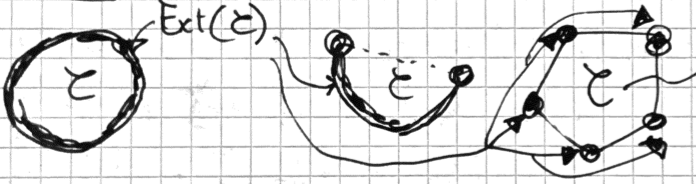
\includegraphics[width=.45\linewidth]{birkhoff/extremal-pts}&
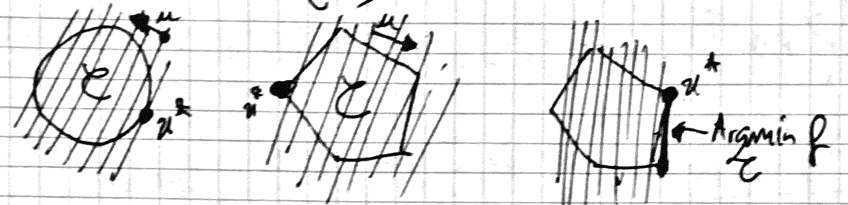
\includegraphics[width=.45\linewidth]{birkhoff/min-cvx}
\end{tabular}
\caption{\label{fig-extremal}
%
Left: extremal points of a convex set. 
Right: the solution of a convex program is a convex set. 
}
\end{figure}


\begin{prop}\label{prop-extr-optim}
	If $\Cc$ is compact, then 
	\eq{
		\text{Extr}(\Cc) \cap \pa{ \uargmin{\P \in \Cc} \dotp{\C}{\P}  } \neq \emptyset.
	}
\end{prop}
\begin{proof}
	One consider $\Ss \eqdef \uargmin{\P \in \Cc} \dotp{\C}{\P}$. 
	%	
	We first note that $\Ss$ is convex (as always for an argmin) and compact, because $\Cc$ is compact and the objective function is continuous, so that $\text{Extr}(\Ss) \neq \emptyset$.
	%
	We will show that $\text{Extr}(\Ss) \subset \text{Extr}(\Cc)$. 
	\todo{finish}
\end{proof}

The following theorem states that the extremal points of bistochastic matrices are the permutation matrices. It implies as a corollary that the cost of Monge and Kantorovitch are the same, and that they share a common solution. 


\begin{thm}[Birkhoff and von Neumann]\label{thm-birkh-vnm}
	One has $\text{Extr}(\Bb_n) = \Pp_n$.
\end{thm}
\begin{proof}
	We first show the simplest inclusion $\Pp_n \subset \text{Extr}(\Bb_n)$. Indeed it follows from the fact that $\text{Extr}([0,1]) = \{0,1\}$. Take $\P \in \Pp_n$, if $\P=(Q+R)/2$ with $Q_{i,j},R_{i,j} \in [0,1]$, since $\P_{i,j} \in \{0,1\}$ then necessarily $Q_{i,j}=R_{i,j} \in \{0,1\}$.
	
	Now we show $\text{Extr}(\Bb_n) \subset \Pp_n$ by showing that $\Pp_n^c \subset \text{Extr}(\Bb_n)^c$ where the complementary are computed inside the larger set $\Bb_n$. So picking $\P \in \Bb_n \backslash \Pp_n$, we need to split $\P = (Q+R)/2$ where $Q,R$ are distinct bistochastic matrices. 
	%
	As shown on figure~\ref{fig-extremal}, $\P$ defines a partite graph linking two sets of $n$ vertices. 
	%
	This graph is composed of isolated edge when $\P_{i,j}=1$ and connected edges corresponding to $0 < \P_{i,j} <1$.
	If $i$ is such a connected vertex on the left (similarly for $j$ on the right), because $\sum_j \P_{i,j}=1$, there is necessarily at least two edges $(i,j_1)$ and $(i,j_2)$ emating from it (similarely on the right there are at least two converging edges $(i_1,j)$ and $(i_2,j)$). This means that by following these connexions, one necessarily can extract a cycle (if not, one could alway extend it by the previous remarks) of the form
	\eq{
		(i_1,j_1,i_2,j_2,\ldots,i_p,j_p), 
		\quad \text{i.e.}\quad i_{p+1}=i_1.
	}
	We assume this cycle is the shortest one among all this (finite) ensemble of cycle. Along this cycle, the left-right and right-left edges satisfy
	\eq{
		0 < \P_{i_s,j_s}, \P_{j_s,i_{s+1}} < 1.
	}
	The $(i_s)_s$ and $(j_s)_s$ are also all distincts because the cycle is the shortest. Lets pick
	\eq{
		\epsilon \eqdef \umin{0 \leq s \leq p} \{ \P_{i_s,j_s}, \P_{j_s,i_{s+1}}, 1-\P_{i_s,j_s}, 1-P_{j_s,i_{s+1}} \}
	}
	so that $0 < \epsilon < 1$. As shown on Figure~\ref{fig-extremal}, right, we split the graph in two set of edges, left-right and right-left
	\eq{
		\Aa \eqdef \{(i_s,j_s)\}_{s=1}^p
		\qandq 
		\Bb \eqdef \{(j_s,i_{s+1})\}_{s=1}^p.
	}
	We define then two matrices as
	\eq{
		Q_{i,j} \eqdef 
		\choice{
			\P_{i,j} \qifq (i,j) \notin \Aa \cup \Bb, \\
			\P_{i,j}+\epsilon/2 \qifq (i,j) \in \Aa, \\
			\P_{i,j}-\epsilon/2 \qifq (i,j) \in \Bb, 		
		}
		\qandq
		R_{i,j} \eqdef 
		\choice{
			\P_{i,j} \qifq (i,j) \notin \Aa \cup \Bb, \\
			\P_{i,j}-\epsilon/2 \qifq (i,j) \in \Aa, \\
			\P_{i,j}+\epsilon/2 \qifq (i,j) \in \Bb, 		
		}.
	}
	Because of the choice of $\epsilon$, one has $0 \leq Q_{i,j}, R_{i,j} \leq 1$.
	Because each left-right edge in $\Aa$ is associated to a right-left edge in $\Bb$, (and the other way) the
	sum constraint on the row (and on the column) is maintain, so that $U,V \in \Bb_n$. Finally, note that $\P=(P+Q)/2$.	
\end{proof}



\begin{figure}
\centering
\begin{tabular}{@{}c@{\hspace{5mm}}c@{}}
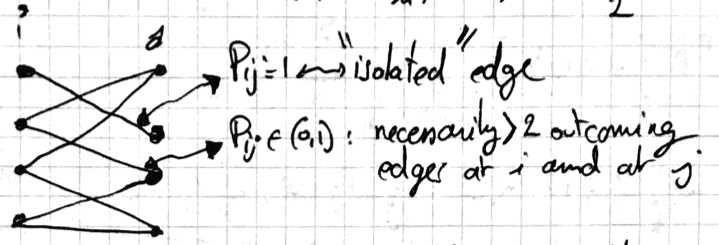
\includegraphics[width=.7\linewidth]{birkhoff/bipartite}&
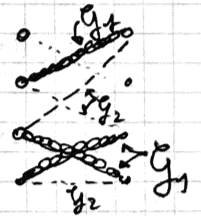
\includegraphics[width=.25\linewidth]{birkhoff/bipartite-split}
\end{tabular}
\caption{\label{fig-extremal}
%%
Left: the support of the coupling $\P$ defines a bipartite graph.
Right: splitting of this graph in two set of edges.
}
\end{figure}

By putting together Proposition~\ref{prop-extr-optim} and Theorem~\ref{thm-birkh-vnm}, one obtains that for the discrete optimal problem with empirical measures, Monge and Kantoritch problems are equivalent.

\begin{cor}[Kantorovich for matching]\label{prop-matching-kanto}
	If $m=n$ and $\a=\b=\ones_n$, then there exists an optimal solution for Problem~\eqref{eq-mk-discr} $\P_{\si^\star}$, which is a permutation matrix associated to an optimal permutation $\si^\star \in \Perm(n)$ for Problem~\eqref{eq-optimal-assignment}.	
\end{cor}

The following proposition shows that these problems result in fact in the same optimum, namely that one can always find a permutation matrix that minimizes Kantorovich's problem~\eqref{eq-mk-discr} between two uniform measures $\a=\b=\ones_n/n$, which shows that the Kantorovich relaxation is \emph{tight} when considered on assignment problems. %Note however that some computational algorithm, which are combinatorial in nature, are dedicated to the case of uniform histograms with the same number of points (see Chapter~\ref{c-algo-basics}). 
%
% Figure~\ref{fig-matching-kantorovitch} shows on the left a 2-D example of optimal matching corresponding to this special case. 

%\begin{figure}
%\centering
%\begin{tabular}{@{}c@{\hspace{5mm}}c@{}}
%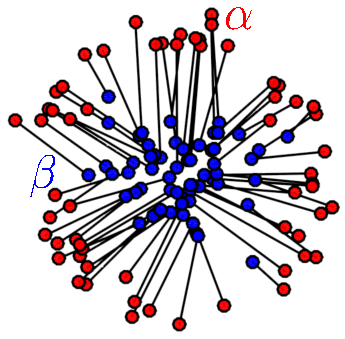
\includegraphics[width=.25\linewidth]{matching-kantorovitch/matching}&
%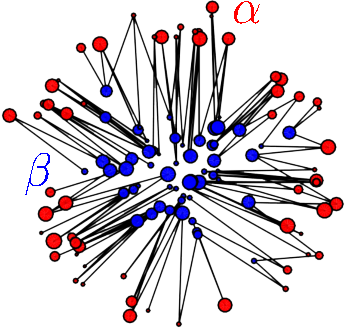
\includegraphics[width=.25\linewidth]{matching-kantorovitch/weighted}
%\end{tabular}
%\caption{\label{fig-matching-kantorovitch}
%%
%Comparison of optimal matching and generic couplings. A black segment between $x_i$ and $y_j$ indicates a non-zero element in the displayed optimal coupling $\P_{i,j}$ solving~\eqref{eq-mk-discr}.
%%
%Left: optimal matching, corresponding to the setting of Proposition~\eqref{prop-matching-kanto} (empirical measures with the same number $n=m$ of points).
%%
%Right: these two weighted point clouds cannot be matched; instead a Kantorovich coupling can be used to associate two arbitrary discrete measures.  
%}
%\end{figure}


\begin{rem}[General case] For general input measure, one does not have equivalence between Monge and Kantorovitch problems (since the Monge constraint is in general empty). But the support of the optimal coupling $\P$ still enjoys some strong regularity, in particular, it defines a cycle-free bipartite graph. This implies in particular that the resulting $\P$ matrix is sparse, for instance one can show that there are always solutions with less than $n+m-1$ non-zero elements.	
\end{rem}

%%%%%%%%%%%%%%%%%%%%%%%%%%%%%%%%%%%%%%%%%%%%%%%%%%%%%%%%%%%%%%%%%%%%%%%%%%%
\subsection{Relaxation for Arbitrary Measures}

%%%
\paragraph{Continuous couplings.}

The definition of $\MK_\c$ in~\eqref{eq-kanto-discr} is extended to arbitrary measures by considering couplings $\pi \in \Mm_+^1(\X \times \Y)$ which are joint distributions over the product space. 
%
The marginal constraint $\P\ones_m=\a, \P\ones_n=\b$ must be replaced by ``integrated'' versions, which are written $\pi_1 = \al$ and $\pi_2 = \be$, where $(\pi_1,\pi_2) \in \Mm(\Xx) \times \Mm(\Yy)$ are the two marginals. 
%
They are defined as $\pi_1 \eqdef P_{1\sharp} \pi$ and $\pi_2 \eqdef P_{2\sharp} \pi$ the two marginals of $\pi$, which are defined using push-forward by the projectors $P_1(x,y)=x$ and $P_2(x,y)=y$.

A heuristic way to understand the marginal constraint $\pi_1 = \al$ and $\pi_2 = \be$, which mimics the discrete case where one sums along the rows and columns is to write
\eq{
	\int_\Yy \d\pi(x,y) = \d\al(x)
	\qandq
	\int_\Xx \d\pi(x,y) = \d\be(y),
}
and the mathematically rigorous way to write this, which corresponds to the change of variables formula, is 
\eq{
	\foralls (f,g) \in \Cc(\Xx) \times \Cc(\Yy), \quad
	\int_{\Xx \times \Yy} f(x) \d\pi(x,y) = \int_\Xx f \d\al
	\qandq
	\int_{\Xx \times \Yy} \d\pi(x,y) = \int_\Yy g \d\be.
}	
%
Using~\eqref{eq-equiv-pushfwd}, these marginal constraints are also equivalent to imposing that $\pi(A \times \Y)=\al(A)$ and $\pi(\X \times B)=\be(B)$ for sets $A \subset \X$ and $B \subset \Y$.

Replacing continuous functions by indicator function, one can also rephrase this conservation of mass constraint as
\eq{
	\foralls (A,B) \in \X \times \Y, \quad
		\pi(A \times \Y) = \al(A)
		\qandq
		\pi(\X \times B) = \be(B). 
}

In the general case, the mass conservation constraint~\eqref{eq-discr-couplings} should thus rewritten as a marginal constraint on joint probability distributions
\eql{\label{eq-coupling-generic}
	\Couplings(\al,\be) \eqdef 
	\enscond{
		\pi \in \Mm_+^1(\X \times \Y)
	}{
		\pi_1 = \al
		\qandq
		\pi_2 = \be
	}.
} 

The discrete case, when $\al=\sum_i \a_i \de_{x_i}$, $\be=\sum_j \a_j \de_{x_j}$, the constraint $\pi_1=\al$ and $\pi_2=\be$ necessarily imposes that $\pi$ is discrete, supported on the set $\{(x_i,y_j)\}_{i,j}$, and thus has the form $\pi = \sum_{i,j} \P_{i,j} \de_{(x_i,y_j)}$. The discrete formulation is thus a special case (and not some sort of approximation) of the continuous formulation. 

The set $\Couplings(\al,\be)$ is always non-empty because it contains at least the tensor product coupling $\al \otimes \be$ defined by $\d(\al\otimes\be)(x,y)=\d\al(x)\d\be(y)$ i.e.
\eq{
	\foralls h \in \Cc(\Xx\times\Yy), \quad
	\int_{\X \times \Y} h(x,y)\d(\al\otimes\be)(x,y) = \int_\X (\int_\Y h(x,y) \d\be(y)) \d\al(x)
	=  \int_\X (\int_\Y h(x,y) \d\al(x) ) \d\be(y).
} 
Indeed, $(\al\otimes\be)_1 = \al$ since
\eq{
	\foralls f \in \Cc(\X), \quad
	\int_\X f(x) \d (\al\otimes\be)_1(x)
	= 
	\int_{\X \times \Y} f(x) d\al(x)\d\be(y)
	= \int_\X f(x) \d\al(x) \int_\Y \d\be
	= \int_\X f(x) \d\al(x)
}
because $\int_\Y \d\be=1$.

A very different (concentrated) type of coupling is defined when there exists a map $T: \X \rightarrow \Y$ such that $T_\sharp \al = \be$ (i.e. the constraint set of Monge's problem~\eqref{eq-monge-continuous} is non-empty). In this case, one has that $\pi = (\Id,T)_\sharp \al \in \Couplings(\al,\be)$. This coupling is defined though the integrated definition of push-forward as
\eq{
	\foralls h \in \Cc(\Xx\times\Yy), \quad
	\int_{\X \times \Y} h(x,y)\d\pi(x,y)
	= 
	\int_{\X} h(x,T(x))\d\al. 
} 
In particular, applying this formula to $h(x,y)=f(x)$ or $h(x,y)=g(y)$  shows that $\pi_1=\al$ and $\pi_2=\be$.



%
%
%\begin{figure}
%\centering
%\begin{tabular}{@{}c@{\hspace{5mm}}c@{\hspace{5mm}}c@{}}
%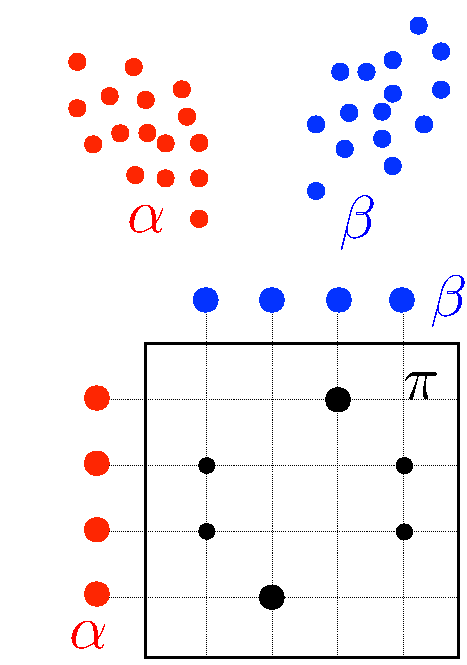
\includegraphics[width=.22\linewidth]{settings/discrete}&
%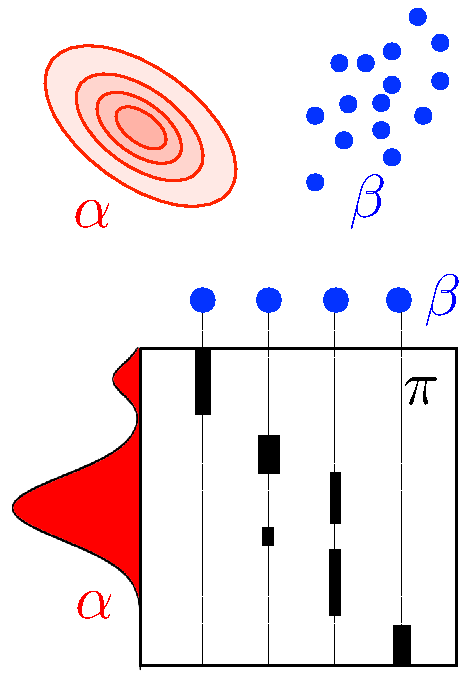
\includegraphics[width=.22\linewidth]{settings/semi-discrete}&
%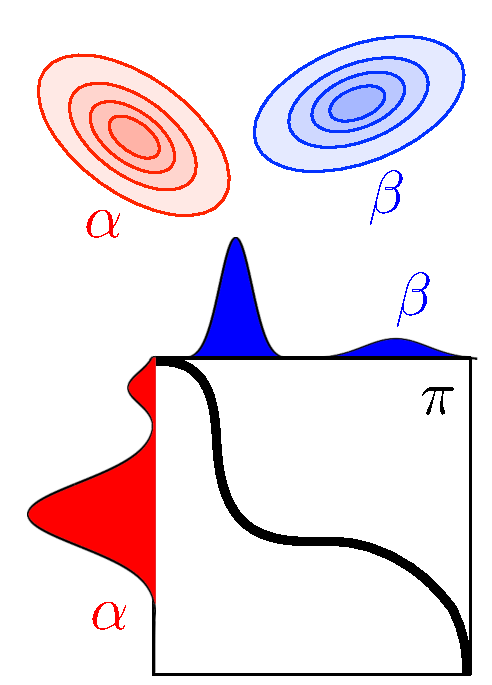
\includegraphics[width=.22\linewidth]{settings/continuous}\\
%Discrete & Semi-discrete & Continuous
%\end{tabular}
%\caption{\label{fig-settings}
%Schematic viewed of input measures $(\al,\be)$ and couplings $\Couplings(\al,\be)$ encountered in the three main scenario for Kantorovich OT. Chapter~\ref{c-algo-semidiscr} is dedicated to the semi-discrete setup.
%}
%\end{figure}


%%%
\paragraph{Continuous Kantorovitch problem.}


The Kantorovich problem~\eqref{eq-kanto-discr} is then generalized as 
\eql{\label{eq-mk-generic}
	\MK_\c(\al,\be) \eqdef 
	\umin{\pi \in \Couplings(\al,\be)}
		\int_{\X \times \Y} \c(x,y) \d\pi(x,y).
}
This is an infinite-dimensional linear program over a space of measures. 


% Figure~\ref{fig-couplings} shows examples of discrete and continuous optimal coupling solving~\eqref{eq-mk-generic}.
% Figure~\ref{fig-couplings-simple} shows other examples of optimal 1-D couplings, involving discrete and continuous marginals.

%\begin{figure}
%\centering
%\begin{tabular}{@{}c@{\hspace{10mm}}c@{}}
%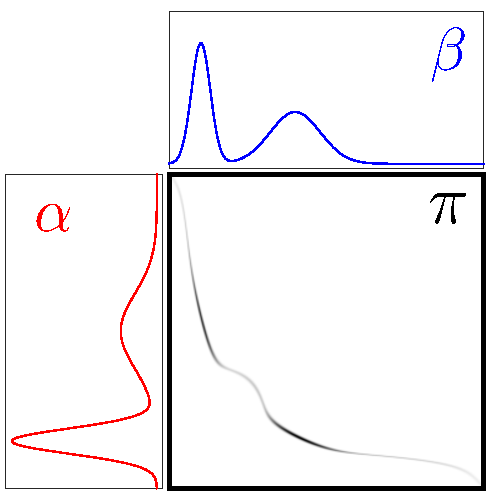
\includegraphics[width=.2\linewidth]{couplings/couplings-continuous}&
%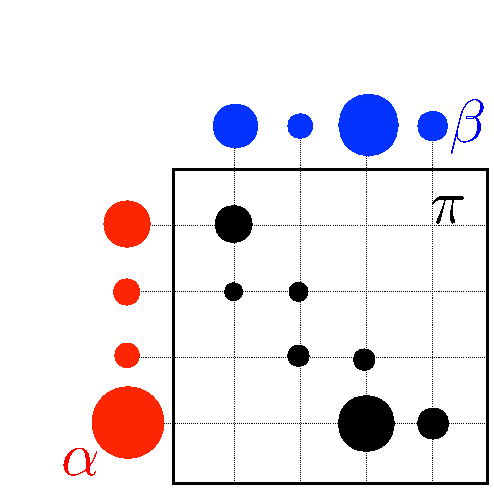
\includegraphics[width=.2\linewidth]{couplings/couplings-discr}
%\end{tabular}
%\caption{\label{fig-couplings}
%Left: ``continuous'' coupling $\pi$ solving~\eqref{eq-coupling-generic} between two 1-D measure with density. The coupling is localized along the graph of the Monge map $(x,\T(x))$ (displayed in black).  
%%
%Right: ``discrete'' coupling $\T$ solving~\eqref{eq-mk-discr} between two discrete measures of the form~\eqref{eq-pair-discr}. The non-zero entries $\T_{i,j}$  are display with a black disk at position $(i,j)$ with radius proportional to $\T_{i,j}$.
%}
%\end{figure}


%\begin{figure}
%\centering
%\begin{tabular}{@{}c@{}c@{}c@{}c@{}}
%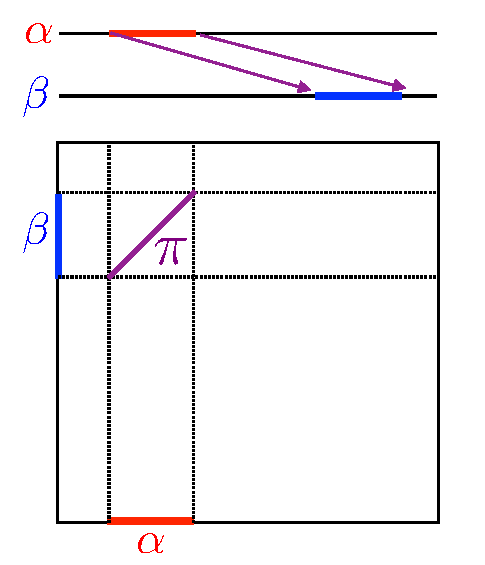
\includegraphics[width=.2\linewidth]{couplings/couplings-1}&
%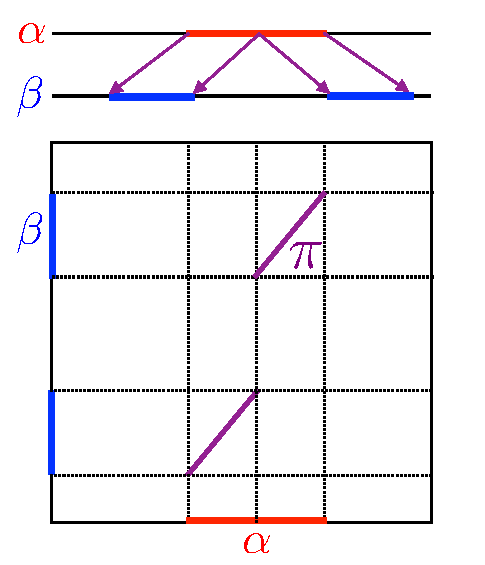
\includegraphics[width=.2\linewidth]{couplings/couplings-2}&
%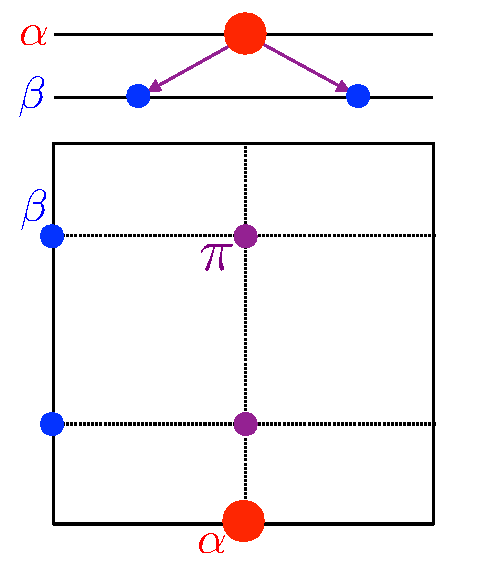
\includegraphics[width=.2\linewidth]{couplings/couplings-3}&
%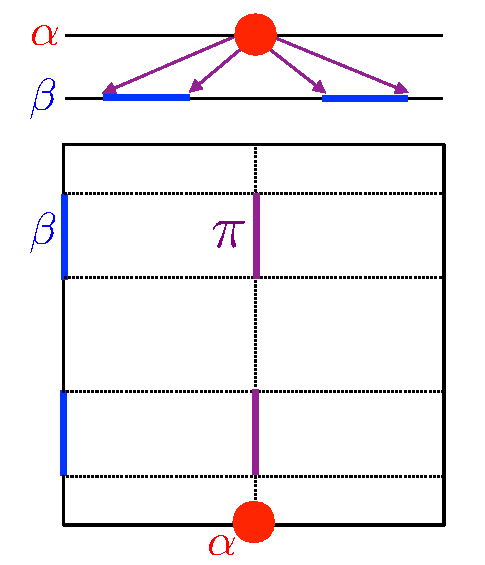
\includegraphics[width=.2\linewidth]{couplings/couplings-4}
%\end{tabular}
%\caption{\label{fig-couplings-simple}
%Four simple examples of optimal couplings between 1-D distributions, represented as maps above (arrows) and couplings below. Inspired by~\cite{Levy2017review}.
%}
%\end{figure}


On compact domain $(\Xx,\Yy)$, \eqref{eq-mk-generic} always has a solution, because using the weak-* topology (so called weak topology of measures), the set of measure is compact, and a linear function with a continuous $c(x,y)$ is weak-* continuous. And the set of constraint is non empty, taking $\al \otimes \be$. On non compact domain, one needs to impose moment condition on $\al$ and $\be$.

%%%%
\paragraph{Probabilistic interpretation.}

If we denote $X \sim \al$ the fact that the law of a random vector $X$ is the probability distribution $\al$, then the marginal constraint appearing in~\eqref{eq-mk-generic} is simply that $\pi$ is the law of a couple $(X,Y)$ and that its coordinates $X$ and $Y$ have laws $\al$ and $\be$. The coupling $\pi$ encodes the statistical dependency between $X$ and $Y$. For instance, $\pi = \al\otimes \be$ means that $X$ and $Y$ are independent, and it unlikely that such a coupling is optimal. Indeed as stated by Brenier's theorem, optimal coupling for a square Euclidean loss on contrary describe totally dependent variable, which corresponds to a coupling of the form $\pi=(\Id,T)_\sharp \al$ in which case $Y=T(X)$ where $T: \X \rightarrow \Y$ is a measurable map. 

With this remark, problem~\eqref{eq-mk-generic} reads equivalently 
\eql{\label{eq-mk-proba}
	\MK_\c(\al,\be) = 
	\umin{X \times \al, Y \sim \be} \EE(c(X,Y)).
}

%%%%
\paragraph{Monge-Kantorovitch equivalence.}

The proof of Brenier theorem~\ref{thm-brenier}  (detailed in Section~\ref{sec-c-transfo}, Remark~\ref{rem-proof-brenier}) to prove the existence of a Monge map actually studies Kantorovitch relaxation (and makes use of duality), and proves that this relaxation is tight in the sense that it has the same cost as Monge problem. 

Indeed, it shows that the support of an optimal $\pi$ is contained in the subdifferential $\partial \phi$ of a convex function $\phi$, which in general is a set-valued mapping \todo{give the example of a segment split into two equally spaced segments}.
%
When $\alpha$ does not have a density, then $\phi$ is non-smooth and non-smooth points where $\al(\{x\})>0$ leads to mass splitting, for instance moving $\de_{0}$ to $(\de_{-1}+\de{+1})/2$ can be achieved using $\phi(x)=|x|$.  


If $\al$ has a density, then this $\phi$ is differentiable $\al$-almost everywhere and we denote $\T=\nabla\phi$ the unique optimal transport (which is a valid definition almost everywhere and one can use any value at point of non differentiability), then the coupling 
\eq{
	\pi = (\Id,\T)_\sharp \al
	\quad\text{i.e.}\quad
	\foralls h \in \Cc(\Xx \times \Yy), \quad
	\int_{\Xx \times \Yy} h \d \pi = \int_{\Xx} h(x,\T(x)) \d\al(x)
}
is optimal.
In term of random vector, denoting $(X,Y)$ a random vector with law $\pi$, it means that any such optimal random vector satisfies $Y=\T(X)$ where $X \sim \al$ (and of course $\T(X) \sim \be$ by the marginal constraint). 


This key result is similar to Birkoff-von-Neumann Theorem~\ref{prop-matching-kanto} in the sense that it provides conditions ensuring the equivalence between Monge and Kantorovitch problems (note however that Birkoff-von-Neumann does not implies uniqueness). Note however that the settings are radically difference (one is fully discrete while the other requires the sources to  be ``continuous'', i.e. to have a density).


%%%%%%%%%%%%%%%%%%%%%%%%%%%%%%%%%%%%%%%%%%%%%%%%%%%%%%%%%%%%%%%%%%%%%%%%%%%
\subsection{Metric Properties}

%%%%
\paragraph{OT defines a distance.}

An important feature of OT is that it defines a distance between histograms and probability measures as soon as the cost matrix satisfies certain suitable properties. Indeed, OT can be understood as a canonical way to lift a ground distance between points to a distance between histogram or measures. 
%
The proof of this result rely on a ``gluing lemma'', which we first prove in the discrete case.

\begin{lem}[Discrete gluing lemma]\label{lem-gluing-discr}
	Given $(\a,\b,\VectMode{c}) \in \simplex_n \times \simplex_p \times \simplex_m$ 
	Let $\P \in \CouplingsD(\a,\b)$ and $\Q \in \CouplingsD(\b,\VectMode{c})$. Then there exists at least a 3-D tensor coupling $\S \in \RR_+^{n \times p \times m}$ 
	such that the 2-D marginals satisfies 
	\eq{
		\sum_{k} \S_{i,j,k} = \P_{i,j}
		\qandq
		\sum_{i} \S_{i,j,k} = \Q_{j,k}.
	}
	Note that this implies that the three 1-D marginals of $\S$ are $(\a,\b,\VectMode{c})$.
\end{lem}
\begin{proof}
	One verifies that
	\eql{\label{eq-glued-discr}
		\S_{i,j,k} = \choice{
			\frac{\P_{i,j} \Q_{j,k}}{\b_j}  \qifq \b_j \neq 0 \\
			0 \text{ otherwise}
		}
	}
	is acceptable. Indeed, if $\b_j \neq 0$
	\eq{
		\sum_{k} \S_{i,j,k} = \sum_{k} \frac{\P_{i,j} \Q_{j,k}}{\b_j} 
		= \frac{\P_{i,j}}{\b_j} ( \Q \ones_m )_j = \frac{\P_{i,j}}{\b_j}  \b_j.
	}
	If $\b_j = 0$, then necessarily $\P_{i,j}=0$ and $\sum_{k} \S_{i,j,k} = 0 = \P_{i,j}$.
\end{proof}

% We first consider the case where, using a term first introduce by~\cite{RubTomGui00}, the ``ground metric'' matrix $\C$ is fixed, representing substitution costs between bins, and shared across several histograms we would like to compare. The following proposition states that OT provides a meaningful distance between histograms supported on these bins.

\begin{prop}\label{prop-metric-histo}
We suppose $n=m$, and that for some $p \geq 1$, $\C=\distD^p=(\distD_{i,j}^p)_{i,j} \in \RR^{n \times n}$ where $\distD \in \RR_+^{n \times n}$ is a distance on $\range{n}$, \emph{i.e.}
\begin{enumerate}% [label=(\roman*)]
	\item $\distD \in \RR_+^{n \times n}$ is symmetric; 
	\item $\distD_{i,j}=0$ if and only if $i=j$; 
	\item $\foralls (i,j,k) \in \range{n}^3, \distD_{i,k} \leq \distD_{i,j}+\distD_{j,k}$.
\end{enumerate}
Then 
\eql{\label{eq-wass-p-disc}
	\WassD_p(\a,\b) \eqdef \MKD_{\distD^p}(\a,\b)^{1/p}
}
(note that $\WassD_p$ depends on $\distD$) defines the $p$-Wasserstein distance on $\Si_n$, \emph{i.e.} $\WassD_p$ is symmetric, positive, $\WassD_p(\a,\b)=0$ if and only if $\a = \b$, and it satisfies the triangle inequality
\eq{
	\foralls \a,\b,\VectMode{c} \in \Si_n, \quad \WassD_p(\a,\VectMode{c}) \leq \WassD_p(\a,\b) + \WassD_p(\b,\VectMode{c}).
}
\end{prop}

\begin{proof}
For the symmetry, since $\distD^p$ is symmetric, we use the fact that if $\P \in \CouplingsD(\a,\b)$ is optimal for $\WassD_p(\a,\b)$, then $\P^\top \in \CouplingsD(\b,\a)$ is optimal for $\WassD_p(\b,\a)$. For the definiteness, since $\C = \distD^p$ has a null diagonal, $\WassD_p(\a,\a)=0$, with corresponding optimal transport matrix $\P^\star=\diag(\a)$; by the positivity of all off-diagonal elements of $\distD^p$, $\WassD_p(\a,\b)>0$ whenever $\a\ne \b$ (because in this case, an admissible coupling necessarily has a non-zero element outside the diagonal). 

To prove the triangle inequality of Wasserstein distances for arbitrary measures, we consider $\a,\b,\VectMode{c} \in\simplex_n$, and let $\P$ and $\Q$ be two optimal solutions of the transport problems between $\a$ and $\b$, and $\b$ and $\VectMode{c}$ respectively. 
%
We use the gluing Lemma~\ref{lem-gluing-discr} which defines $\S \in \RR_+^{n^3}$ with marginals $\sum_{k}\S_{\cdot,\cdot,k}=\P$ and $\sum_i \S_{i,\cdot,\cdot}=\Q$. We define $\R=\sum_{j}\S_{\cdot,j,\cdot}$, which is an element of $\CouplingsD(\a,\VectMode{c})$. Note that if one assumes $\b>0$ then $\R = \P \diag(1/\b) \Q$.
%

The triangle inequality follows from
$$\begin{aligned}
\WassD_p(\a,\VectMode{c})&=\Big(\min_{\tilde\R\in \CouplingsD(\a,\VectMode{c})}\dotp{\tilde\R}{\distD^p}\Big)^{1/p} \leq \dotp{\R}{\distD^p}^{1/p}\\
&= \Big(\sum_{i,j,k}  \distD^p_{ik}\sum_{j} \S_{i,j,k} \Big)^{1/p} 
 \leq \Big(\sum_{i,j,k} \left(\distD_{ij}+\distD_{j,k}\Big)^p  \S_{i,j,k} \right)^{1/p} \\
& \leq \Big(\sum_{i,j,k} \distD^p_{ij} \S_{i,j,k} \Big)^{1/p} + \Big(\sum_{i,j,k}\distD^p_{j,k} \S_{i,j,k} \Big)^{1/p} \\
&= \Big(\sum_{i,j} \distD^p_{i,j}  \sum_k \S_{i,j,k} \Big)^{1/p} + \Big(\sum_{j,k} \distD^p_{j,k}  \sum_i \S_{i,j,k} \Big)^{1/p}\\
&= \Big(\sum_{i,j} \distD^p_{i,j}\P_{i,j}\Big)^{1/p} + \Big(\sum_{j,k} \distD^p_{j,k} \Q_{j,k}\Big)^{1/p} 
= \WassD_p(\a,\b) +\WassD_p(\b,\b).
\end{aligned}
$$
%
The first inequality is due to the sub-optimality of $\SS$, the second is the usual triangle inequality for elements in $\distD$, and the third comes from Minkowski's inequality.
\end{proof}

Proposition~\ref{prop-metric-histo} generalizes from histogram to arbitrary measures that need not be discrete. For this, one needs the following general gluing lemma.

\begin{lem}[Gluing lemma]\label{lem-gluing-general}
	Let $(\al,\be,\ga) \in \Mm_+^1(\Xx) \times \Mm_+^1(\Yy) \times \Mm_+^1(\Yy)$
	where $(\Xx,\Yy,\Zz)$ are three polish spaces (i.e. separable topological space which can be metrized using a distance which makes it a complete metric space).  
	%
	Given $\pi \in \Couplings(\al,\be)$ and $\xi \in \Couplings(\be,\ga)$, then there exists at least a tensor coupling measure
	$\sigma \in \Mm_+(\Xx \times \Yy \times \Zz)$ such that 
	\eq{
		(P_{\Xx,\Yy})_\sharp \sigma = \pi
		\qandq
		(P_{\Yy,\Zz})_\sharp \sigma = \xi
	}
	where we denoted the projector $P_{\Xx,\Yy}(x,y,z)=(x,y)$ and $P_{\Yy,\Zz}(x,y,z)=(y,z)$. 
\end{lem}
\begin{proof}
	The proof of this fundamental result is involved since it requires using the disintegration of measure (which corresponds to conditional probabilities). 
	%
	The disintegration of measures is applicable because the spaces are polish. 
	%
	We disintegrate $\pi$ and $\xi$ against $\be$ to obtain two families $(\pi_y)_{y \in \Yy}$ and $(\xi_y)_{y \in \Yy}$ of probability distributions on $\Xx$ and $\Zz$. These families are defined by the fact that 
	\eq{
		\foralls h \in \Cc(\Xx \times \Yy), \quad 
		\int_\Yy \Big( \int_\Xx h(x,y) \d \pi_y(x) \Big) \d \be(y) = \int h(x,y) \d\pi(x,y).
	}
	and similarly for $\xi$.
	%
	When $\be=\sum_i \b_j \de_{y_j}$ and $\pi=\sum_{i,j}P_{i,j} \de_{y_j}$, then this conditional distribution is defined on the support of $\be$ as
	$\pi_{y_j} = \sum_i \frac{\P_{i,j}}{\b_j} \de_{x_i}$ (and similarly for $\xi$).
	%
	Then one defines the glued measure informally $``\sigma(x,y,z) = \pi_y(x) \xi_y(z) \be(y)''$, which formally reads
	\eq{
		\foralls g \in \Cc(\Xx \times \Yy \times \Zz), \quad
		\int g(x,y,z) \d\sigma(x,y,z) = \int g(x,y,z) \d \pi_y(x) \d \xi_y(z) \d \be(y).
	}
	For discrete measures, this matches the definition~\eqref{eq-glued-discr}, since $\sigma=\sum_{i,j,k} \S_{i,j,k} \de_{x_i,y_j,z_k}$ where
	\eq{
		\S_{i,j,k} = \frac{\P_{i,j}}{\b_j} \frac{\Q_{j,k}}{\b_j} \b_j.
	}
\end{proof}

Using this gluing lemma, we can now construct the Wasserstein distance in the general setting of arbitrary distributions on a Polish space.

\begin{prop}\label{prop-metric-measure}
We assume $\X=\Y$, and that for some $p \geq 1$, $\c(x,y)=\dist(x,y)^p$ where $\dist$ is a distance on $\X$, \emph{i.e.} \\
	\hbox{}\qquad (i) $\dist(x,y) = \dist(y,x) \geq 0$;  \\
	\hbox{}\qquad (ii)  $\dist(x,y)=0$ if and only if $x=y$;  \\
	\hbox{}\qquad (ii)  $\foralls (x,y,z) \in \X^3, \dist(x,z) \leq \dist(x,y)+\dist(y,z)$. \\
Then 
\eql{\label{eq-defn-wass-dist}
	\Wass_p(\al,\be) \eqdef \MK_{\dist^p}(\al,\be)^{1/p}
}
(note that $\Wass_p$ depends on $\dist$) defines the $p$-Wasserstein distance on $\X$, \emph{i.e.} $\Wass_p$ is symmetric, positive, $\Wass_p(\al,\be)=0$ if and only if $\al = \be$, and it satisfies the triangle inequality
\eq{
	\foralls (\al,\be,\ga) \in  \Mm_+^1(\X)^3, \quad \Wass_p(\al,\ga) \leq \Wass_p(\al,\be) + \Wass_p(\be,\ga).
}
\end{prop}

\begin{proof}
	The symmetry follows from the fact that since $d$ is symmetric, if $\pi(x,y)$ is optimal for $\MK_{\dist^p}(\al,\be)$, then 
	$\pi(y,x) \in \Couplings(\be,\al)$ is optimal for $\MK_{\dist^p}(\be,\al)$. 
	%
	If $\MK_{\dist^p}(\al,\be)=0$, then necessarily an optimal coupling $\pi$ is supported on the diagonal $\De \eqdef \{(x,x)\}_x \subset \Xx^2$.
	%
	We denote $\la(x)$ the corresponding measure on the diagonal, i.e. such that $\int h(x,y) \d\pi(x,y) = \int h(x,x) \d \la(x)$.
	%
	Then since $\pi \in \Couplings(\al,\be)$ necessarily $\la=\al$ and $\la=\be$ so that $\al=\be$.
	
	For the triangle inequality, we consider optimal couplings $\pi \in \Couplings(\al,\be)$ and $\xi \in \Couplings(\be,\ga)$
	and we glue them according to the Lemma~\ref{lem-gluing-general}.
	%
	We define the composition of the two couplings $(\pi,\xi)$ as $\rho \eqdef (P_{\Xx,\Zz})_\sharp \si$.
	%
	Note that if $\pi$ and $\xi$ are coupling induced by two Monge maps $T_\Xx(x)$ and $T_\Yy(y)$, then $\rho$ is itself induced by the Monge map $T_\Yy \circ T_\Xx$, so that this notion of composition of coupling generalizes the composition of maps.
	%
	The triangular inequality follows from  
	$$\begin{aligned}
		\Wass_p(\al,\ga) & \leq \Big( \int_{\Xx \times \Zz} \dist(x,z)^p \d\rho(x,z)\Big)^{1/p}  
		= \Big( \int_{\Xx \times \Yy \times \Zz} \dist(x,z)^p \d\si(x,y,z)\Big)^{1/p}		\\
		 &\leq \Big( \int_{\Xx \times \Yy \times \Zz} (\dist(x,y)+\dist(y,z))^p \d\si(x,y,z)\Big)^{1/p} \\
		 &\leq \Big( \int_{\Xx \times \Yy \times \Zz} \dist(x,y)^p \d\si(x,y,z)\Big)^{1/p}
		    +  \Big( \int_{\Xx \times \Yy \times \Zz} \dist(y,z)^p \d\si(x,y,z)\Big)^{1/p} \\
		  &= \Big( \int_{\Xx \times \Yy} \dist(x,y)^p \d\pi(x,y,z)\Big)^{1/p}
		    +  \Big( \int_{\Yy \times \Zz} \dist(y,z)^p \d\xi(y,z)\Big)^{1/p}
		    = \Wass_p(\al,\be)  + \Wass_p(\be,\ga) .
	\end{aligned}$$
\end{proof}

This distance $\Wass_p$ defined though Kantorovitch problem~\eqref{eq-defn-wass-dist} should be contrasted with the distance $\tilde\Wass$ obtained using Monge's problem~\eqref{eq-monge-distance}. Kantorovitch distance is always finite, while Monge's one might be infinite if the constraint set $\enscond{T}{T_\sharp \al=\be}$ is empty. In fact, one can show that as soon as this constraint set is non-empty, and even if no optimal $T$ exists, then one has $\Wass_p = \tilde\Wass_p$, which is a non-trivial result. Kantorovitch distance should thus be seen as a (convex) relaxation of Monge's distance, which behave in a much nicer way, as we will explore next (it is continuous with respect to the convergence in law topology.


%%%%
\paragraph{Convergence in law topology.}

Let us first note that on a compact space, all $W_p$ distance defines the same topology (although they are not equivalent, the notion of converging sequence is the same).

\begin{prop}\label{prop-comp-wass-p}
	On a compact space $\Xx$, one has for $p \leq q$
	\eq{
		W_p( \al,\be ) \leq W_q(\al,\be) \leq \text{\upshape diam}(\Xx)^{\frac{q-p}{q}} W_p(\al,\be)^{\frac{q}{p}}
	}
\end{prop}
\begin{proof}
	The left inequality follows from Jensen inequality, $\phi(\int c(x,y) \d\pi(x,y)) \leq \int \phi(c(x,y)) \d\pi(x,y)$, applied to any probability distribution $\pi$ and to the convex function $\phi(r)=r^{q/p}$ to $c(x,y)=\norm{x-y}^p$, so that one gets
	\eq{
		\pa{\int \norm{x-y}^{p} \d\pi(x,y)}^{\frac{q}{p}} \leq \int \norm{x-y}^{q} \d\pi(x,y).
	} 	
	The right inequality follows from
	\eq{
		\norm{x-y}^q \leq \text{diam}(\Xx)^{q-p} \norm{x-y}^p.
	}
\end{proof}

The Wasserstein distance $\Wass_p$ has many important properties, the most important one being that it is a weak distance, \emph{i.e.} it allows to compare singular distributions (for instance discrete ones) and to quantify spatial shift between the supports of the distributions. This corresponds to the notion of weak$^*$ convergence.

\begin{defn}[Weak$^*$ topology]\label{dfn-weak-conv}
	$(\al_k)_k$ converges weakly$^*$ to $\al$ in $\Mm_+^1(\Xx)$ (denoted $\al_k \rightharpoonup \al$) if and only if for any continuous function $f \in \Cc(\Xx)$, $\int_\Xx f \d\al_k \rightarrow \int_\Xx f \d\al$.
\end{defn}

In term of random vectors, if $X_n \sim \al_n$ and $X \sim \al$ (not necessarily defined on the same probability space), the weak$^*$ convergence corresponds to the convergence in law of $X_n$ toward $X$.

\begin{defn}[Strong topology]
The simplest distance on Radon measures is the total variation norm, which is the dual norm of the $L^\infty$ norm on $\Cc(\Xx)$ and whose topology is often called the ``strong'' topology
\eq{
	\norm{\al-\be}_{TV} \eqdef \usup{\norm{f}_\infty \leq 1} \int f \d(\al-\be)
	 = |\al-\be|(\Xx)
}
where $|\al-\be|(\Xx)$ is the mass of the absolute value of the difference measure. When $\al-\be=\rho \d x$ has a density, then $\norm{\al-\be}_{TV}=\int |\rho(x)| \d x=\norm{\rho}_{L^1(\d x)}$ is the $L^1$ norm associated to $\d x$. When $\al-\be=\sum_i u_i \de_{z_i}$ is discrete, then $\norm{\al-\be}_{TV}=\sum_i |u_i|=\norm{u}_{\ell^1}$ is the discrete $\ell^1$ norm. 
\end{defn}

In the special case of Diracs, having $\int f \d\de_{x_n} = f(x_n) \rightarrow \int f \d\de_{x} = f(x)$ for any continuous $f$ is equivalent to $x_n \rightarrow x$. One can then contrast the strong topology with the Wasserstein distance, if $x_n \neq x$, 
\eq{
	\norm{\de_{x_n}-\de_x}_{TV}=2
	\qandq
	W_p(\de_{x_n},\de_x) = d(x_n,x).
}
This shows that for the strong topology, Diracs never converge, while they do converge for the Wasserstein distance. In fact it is a powerful property of the Wasserstein distance, which is regular with respect to the weak$^*$ topology, and metrizes it.

\begin{prop}
	If $\Xx$ is compact, $\al_k \rightharpoonup \al$ if and only if $W_p(\al_k,\al) \rightarrow 0$. 
\end{prop}

The proof of this proposition requires the use of duality, and is delayed to later, see Proposition~\ref{cor-topol-wass}. 
On non-compact spaces, one needs also to impose the convergence of the moments up to order $p$.
%
Note that there exists alternative distances which also metrize weak convergence. The simplest one are Hilbertian kernel norms, which are detailed in Section~\ref{sec-dual-norms}.

Another example of such a weak convergence is the fact that on $\Xx=\RR$
\eq{
	\frac{1}{n} \sum_{k=1}^n \de_{k/n} \rightharpoonup \Uu_{[0,1]}
}
(convergence toward the uniform measure on $[0,1]$), which comes from the convergence of Riemann sums 
\eq{
	\foralls f \in \Cc(\RR), \quad
	\frac{1}{n} \sum_{k=1}^n f(k/n) \longrightarrow \int_0^1 f(x) \d x.
}
In contrary, one has that for all $n$, since the two measure are mutually singular
\eq{
	\norm{ \frac{1}{n} \sum_{k=1}^n \de_{k/n} - \Uu_{[0,1]}}_{TV} = 
	\norm{ \frac{1}{n} \sum_{k=1}^n \de_{k/n} }_{TV} +  \norm{\Uu_{[0,1]}}_{TV} = 2
}
so that there is no strong convergence. 


 
 
%%%%%
\paragraph{Applications and implications}

Applications for having a geometric distance : barycenters, shape registration loss functions, density fitting